% Created 2013-04-18 Thu 19:42
\documentclass[11pt,presentation]{beamer}
\usepackage[utf8]{inputenc}
\usepackage[T1]{fontenc}
\usepackage{fixltx2e}
\usepackage{graphicx}
\usepackage{longtable}
\usepackage{float}
\usepackage{wrapfig}
\usepackage{soul}
\usepackage{textcomp}
\usepackage{marvosym}
\usepackage[nointegrals]{wasysym}
\usepackage{latexsym}
\usepackage{amssymb}
\usepackage{hyperref}
\tolerance=1000
\AtBeginSection[]{\begin{frame}<beamer>\frametitle{提纲}\tableofcontents[currentsection]\end{frame}}
\providecommand{\alert}[1]{\textbf{#1}}

\title{大数据环境下信息抽取模板自动聚类与发现}
\author{计92 丘骏鹏 2009011282}
\date{指导老师:朱小燕~郝宇}
\hypersetup{
  pdfkeywords={},
  pdfsubject={},
  pdfcreator={Emacs Org-mode version 7.8.11}}

\usetheme{default}\usecolortheme{default}
\usepackage{listings}\usepackage{fontspec}\usepackage{xunicode}\usepackage{xltxtra}\usepackage{xeCJK}
\setmainfont{Times New Roman}\setmonofont{Courier New}\setCJKmainfont[BoldFont=YouYuan]{SimSun}\setCJKfamilyfont{song}{SimSun}\setCJKfamilyfont{msyh}{微软雅黑}\setCJKfamilyfont{fs}{FangSong}
\begin{document}

\maketitle



\begin{frame}<beamer>\frametitle{提纲}\tableofcontents\end{frame}
\section{选题回顾}
\label{sec-1}
\begin{frame}[fragile]
\frametitle{背景}
\label{sec-1-1}

\begin{itemize}
\item 已经获取到海量的新闻、博客、论坛等网页原始数据,需要从中提取结构化的信息
\item 从已有数据中抽取模板,利用模板去抽取相似网页中的信息。
\item 新的网页可能采取新的模板,需要自动检测,分类和抽取这些新的模板
\item 目标:提取结构化信息,如新闻中的标题和正文,博客的标题和内容等,用于后续的处理。
  \tiny

\lstset{extendedchars=false,basicstyle=\ttfamily\footnotesize,escapechar=`,breaklines,language=nxml}
\begin{lstlisting}
<document>
  <news>
    <title>foobar</title>
    <content>blablabla</content>
  </news>
</document>
\end{lstlisting}
\end{itemize}
\end{frame}
\begin{frame}[fragile]
\frametitle{输入}
\label{sec-1-2}
\begin{itemize}

\item 文档集合\\
\label{sec-1-2-1}%
\lstset{extendedchars=false,basicstyle=\ttfamily\footnotesize,escapechar=`,breaklines,language=HTML}
\begin{lstlisting}
  <html>                |  <html>
    <body>              |    <body>
      <h1>Title1</h1>   |      <h1>Title2</h1>
      <p>Content1</p>   |      <p>Content2</p>
    </body>             |    </body>
  </html>               |  </html>
------------------------|--------------------------
  <html>                |  <html>
    <body>              |    <body>
      <div>             |      <div>
        <div>foo1</div> |        <div>foo2</div>
        <div>bar1</div> |        <div>bar2</div>
      </div>            |      </div>
    </body>             |    </body>
  </html>               |  </html>
\end{lstlisting}

\end{itemize} % ends low level
\end{frame}
\begin{frame}[fragile]
\frametitle{输出}
\label{sec-1-3}
\begin{columns}[t]
\begin{column}{0.5\textwidth}
\begin{itemize}

\item 抽取的模板1\\
\label{sec-1-3-1}%
\lstset{extendedchars=false,basicstyle=\ttfamily\footnotesize,escapechar=`,breaklines,language=HTML}
\begin{lstlisting}
<html>
  <body>
    <h1>?</h1>
    <p>?</p>
  </body>
</html>
\end{lstlisting}
\end{itemize} % ends low level
\end{column}
\begin{column}{0.5\textwidth}
\begin{itemize}

\item 抽取的模板2\\
\label{sec-1-3-2}%
\lstset{extendedchars=false,basicstyle=\ttfamily\footnotesize,escapechar=`,breaklines,language=HTML}
\begin{lstlisting}
<html>
  <body>
    <div>
      <div>?</div>
      <div>?</div>
    </div>
  </body>
</html>
\end{lstlisting}

\end{itemize} % ends low level
\end{column}
\end{columns}
\end{frame}
\section{系统设计与实现}
\label{sec-2}
\begin{frame}
\frametitle{框架}
\label{sec-2-1}
\begin{columns}[t]
\begin{column}{0.3\textwidth}
%% \textbf{:BMCOL:B\_ignoreheading:}
\label{sec-2-1-1}

整体框架示意图
\end{column}
\begin{column}{0.7\textwidth}
%% \textbf{:B\_ignoreheading:BMCOL:}
\label{sec-2-1-2}

    \begin{figure}[htb]
    \centering
    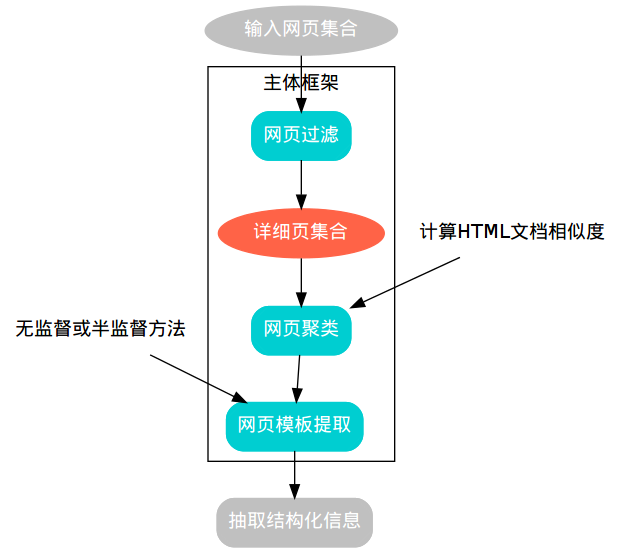
\includegraphics[width=20em,angle=0]{./framework.png}
    \caption{\label{fig:1}framework}
    \end{figure}
\end{column}
\end{columns}
\end{frame}
\begin{frame}
\frametitle{系统实现概况}
\label{sec-2-2}
\begin{itemize}

\item 实现语言\\
\label{sec-2-2-1}%
Java+\href{http://en.wikipedia.org/wiki/Scala_(programming_language)}{Scala}。Scala是JVM上的静态类型语言,可以和Java之间无缝操作,支持面向对象
    和函数式等编程范式。

\item 使用的第三方库
\label{sec-2-2-2}%
\begin{enumerate}
\item \href{http://site.icu-project.org/}{icu4j} : 用于检测网页字符编码
\item \href{http://jsoup.org}{Jsoup} : HTML Parser。可以自定义Visitor来访问树的节点。
\item \href{https://github.com/twitter/util}{util-logging} : twitter包装的java.util.logging库,用于日志系统
\item \href{https://github.com/typesafehub/config}{typesafe's config} : 完成配置文件读取
\item \href{http://akka.io}{akka} : Java \& Scala的Actor模型库
\end{enumerate}


\item 主要模块实现
\label{sec-2-2-3}%
\begin{itemize}
\item $\boxtimes$ 网页过滤
\item $\boxtimes$ 网页聚类
\item $\Box$ 模板抽取
\end{itemize}
\end{itemize} % ends low level
\end{frame}
\begin{frame}
\frametitle{系统设计(1)}
\label{sec-2-3}
\begin{itemize}

\item 实验数据统计\\
\label{sec-2-3-1}%
\begin{center}
\begin{tabular}{llll}
           &  blog   &  news   &  other   \\
\hline
 文件个数  &  59998  &  81561  &  183635  \\
 总大小    &  5.4G   &  7.9G   &  18G     \\
\end{tabular}
\end{center}



前期主要针对blog数据做了一些实验

\end{itemize} % ends low level
\end{frame}
\begin{frame}[fragile]
\frametitle{系统设计(2)}
\label{sec-2-4}
\begin{itemize}

\item 过滤目录页
\label{sec-2-4-1}%
\begin{itemize}
\item 新浪博客的目录页和详细页可以用URL区分。比如某个博主的目录页为
  \tiny

\begin{verbatim}
http://blog.sina.com.cn/u/1439351555
\end{verbatim}
  \normalsize
  他的某篇文章的URL格式为
  \tiny

\begin{verbatim}
http://blog.sina.com.cn/s/blog_55cac30301016yb1.html
\end{verbatim}
  \normalsize
  因此对于博客数据可以用URL正则进行过滤
\item 通过shell命令进行统计后,得到的结果为:blog中不带html后缀的文件有23430,带有
  html后缀的文件有36568。过滤出blog数据中有用的详细页数据为36568。
\end{itemize}

\end{itemize} % ends low level
\end{frame}
\begin{frame}[fragile]
\frametitle{系统设计(3)}
\label{sec-2-5}
\begin{itemize}

\item 预处理\\
\label{sec-2-5-1}%
接下来我们需要对详细页进行预处理。
\begin{itemize}
\item 去除空行
\item 去除无用标签

\begin{verbatim}
<script>, <link>, <style>, <br>, <img>, <em>
\end{verbatim}
\item 去除标签属性值,加速Dom Tree的构建速度
\item 去除文本 \texttt{<\#text>} 和 \texttt{CDATA} 数据,只保留结构化的标签名
\item 将树结构平坦化:遍历Dom Tree得到TreeNode序列,在每个TreeNode保存节点的名字和深度
\end{itemize}
\end{itemize} % ends low level
\end{frame}
\begin{frame}
\frametitle{系统设计(4)}
\label{sec-2-6}
\begin{itemize}

\item 近似度计算\\
\label{sec-2-6-1}%
为了方便计算以及后续的模板的抽取,采用LCS作为计算相似度的基础
\begin{eqnarray*}
  c(i)(j) =
  \begin{cases}
    0 & i = 0,\: j = 0\\
    c(i-1)(j-1) + 1 & i,\: j > 0, x_i=y_j\\
    \max(c(i)(j-1), c(i-1)(j)) & i, j > 0,\: x_i \ne y_j
  \end{cases}
\end{eqnarray*}

\item Longest Common Tag Subsequence\\
\label{sec-2-6-2}%
\[
d_{LCTS}(D_1,D_2)=1-\frac{|lcts(D_1,D_2)|}{\max(|D_1|,|D_2|)}
\]

\end{itemize} % ends low level
\end{frame}
\begin{frame}
\frametitle{系统优化}
\label{sec-2-7}

\begin{enumerate}
\item LCS的动态规划算法的时间复杂度为 \texttt{O(mn)} ,空间复杂度也是 \texttt{O(mn)} ,需要做一定
   的优化。
\item 假设每运行一次算法的时间为t,以最小的文档集合blog为输入(数目约为60000篇),则
   计算文档集合中两两之间距离的总时间约为:
   \[
   \frac{60000^2}{2 * 3600}*t=5*10^5*t
   \]
   取\(t=0.001s\),则总时间为\(5*10^5*0.001=500h\)。
\item 文档数很大,运行时需载入内存,也需要尽量减少空间复杂度
\end{enumerate}
\end{frame}
\begin{frame}
\frametitle{优化内存}
\label{sec-2-8}

\begin{itemize}
\item 动态规划原理式
     \begin{eqnarray*}
       c(i)(j) =
       \begin{cases}
         0 & i = 0,\: j = 0\\
         c(i-1)(j-1) + 1 & i,\: j > 0, x_i=y_j\\
         \max(c(i)(j-1), c(i-1)(j)) & i, j > 0,\: x_i \ne y_j
       \end{cases}
     \end{eqnarray*}
     以行优先遍历为例:实际上我们在计算每一个点的值时,依赖的信息只包括这一行之
     前已计算出的点和前一行的点,所以只需要两个一维数组即可。空间复杂度降低为
     \texttt{O(n)} 。
\end{itemize}
\end{frame}
\begin{frame}[fragile]
\frametitle{优化时间}
\label{sec-2-9}

\begin{itemize}
\item 本身HTML文档的表示方式是有冗余的。如果每个HTML标签都有对应的开始和结束标签,
     那么每一对这样的标签 \texttt{<tagName></tagname>} 可以用 \texttt{(tagName, depth)} 来表示。
\item 类比:\href{http://en.wikipedia.org/wiki/S-expression}{S-expression} 。可以将严格的XML转换为S-expression而无信息丢失,因此只需
     要记录当前括号包含的第一个符号的名字(对应与tagName)和嵌套层数(对应于深度)
     \tiny

\lstset{extendedchars=false,basicstyle=\ttfamily\footnotesize,escapechar=`,breaklines,language=Lisp}
\begin{lstlisting}
<html>                          <=>  (html           
 <body>                         <=>    (body         
  <div>                         <=>      (div        
   <p></p></div></body></html>  <=>        (p))))
\end{lstlisting}
     \normalsize
\item 用途:减少tag序列长度,只保留开始tag和深度即可。大部分的标签都是成对的,因此
     这样大概可以减少一半的tag序列长度。
\item 标签名hash:直接比较计算好标签的hash值,避免字符串比较
\end{itemize}
\end{frame}
\begin{frame}
\frametitle{优化计算方式(1)}
\label{sec-2-10}

\begin{itemize}
\item 在以上优化的基础上,两两之间进行一次计算需要的时间为\(0.001\sim 0.002s\)。
\item 之前已经计算过,在\(t=0.001s\)的情况下,计算一次blog集合中所有文档相互之间
     的距离需要500小时。
\item 优化计算方式:采用多线程进行计算。
\end{itemize}
\end{frame}
\begin{frame}
\frametitle{优化计算方式(2)}
\label{sec-2-11}
\begin{itemize}

\item 采用Actor库进行实现
\label{sec-2-11-1}%
\begin{itemize}
\item 一种并行计算的模型,与上世纪70年代提出
\item 在Actor模型里,每个Actor是完全独立的,相互间采用异步、非阻塞的消息传递进行
      通信
\item 比多线程的优点:可以避免使用全局状态、锁、信号量等一些低级的同步原语;有封
      装好的线程调度算法,不需要手动对线程进行管理,简化任务的分割。
\end{itemize}


\end{itemize} % ends low level
\end{frame}
\begin{frame}
\frametitle{优化计算方式(3)}
\label{sec-2-12}
\begin{itemize}

\item 具体实现
\label{sec-2-12-1}%
\begin{itemize}
\item 计算一个文档集合两两之间的相似度相当于计算一个正方形的上半部分的三角形区域。
\item 将该区域用等距的横线和纵线分割,然后将这些区域通过调度器分发给每个可用的Actor
  进行计算。调度算法采用简单的Round-Robin。
\end{itemize}

\end{itemize} % ends low level
%% \textbf{:B\_ignoreheading:BMCOL:}
\label{sec-2-12-2}

\begin{figure}[htb]
\centering
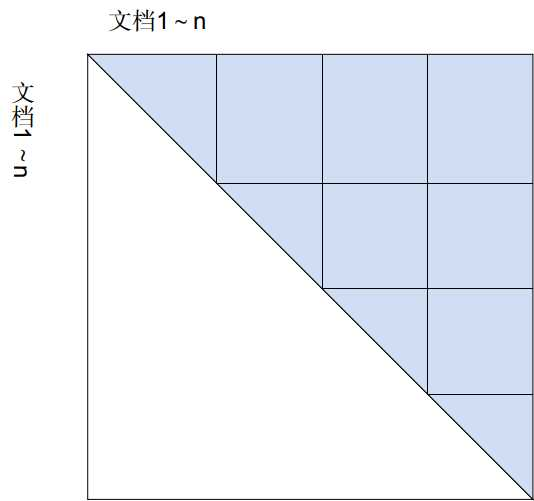
\includegraphics[width=0.35\textwidth,angle=0]{./图片1.jpg}
\caption{\label{fig:1}示意图}
\end{figure}
\end{frame}
\begin{frame}
\frametitle{聚类算法}
\label{sec-2-13}
\begin{itemize}

\item 实现了一个最简单的层次聚类算法
\label{sec-2-13-1}%

\item 过程
\label{sec-2-13-2}%
\begin{itemize}
\item 每个文档开始时单独为一类
\item 选择中心点距离最近的两个类进行合并
\item 更新类中心点:选择距离其他点距离之和最小的点作为类的新中心点,重复以上过程
\end{itemize}

\item 算法特点
\label{sec-2-13-3}%
\begin{itemize}
\item 只需要计算一次文档集合相互之间的相似度
\item 阈值较难设置
\end{itemize}

\end{itemize} % ends low level
\end{frame}
\section{初步结果}
\label{sec-3}
\begin{frame}
\frametitle{初步实验概况}
\label{sec-3-1}

\begin{itemize}
\item 目前只在实验室的电脑上进行过实验,机器配置为16个逻辑CPU+24G内存,尚未部署到
  Hadoop上。
\item 由于以上限制,目前小数据量上做过实验:从blog中抽取出了1000个文档作为文档集合
\item 计算相似度时间:约100s
\item 聚类所需时间:约10s
\end{itemize}
\end{frame}
\begin{frame}
\frametitle{初步实验结果}
\label{sec-3-2}

\begin{itemize}
\item 阈值为0.1时,聚成71类,效果很差
\item 阈值为0.5时,聚成8类;同一博主的文章大部分被分成同一类,但也有分错
\item 阈值为0.7时,聚成2类;通过手工检查,两个类别仍有分错现象
\item 阈值为0.9时,聚成1类;比较符合目前手工检查的结果
\end{itemize}
\end{frame}
\begin{frame}
\frametitle{初步分析}
\label{sec-3-3}

\begin{itemize}
\item 由于目前只能人工一个个检查实验结果进行评价,还缺乏比较系统可行的评价指标,以上
  结果也并不是非常全面
\item 阈值难以设置,目前需人工修改,并不断检查来判断好坏
\item 从聚类的结果来看,目前采用LCS的算法计算相似度效果不算非常好,在阈值为0.7时聚成
  2类时有相似网页聚类错误的情况
\end{itemize}
\end{frame}
\section{问题及后期工作}
\label{sec-4}
\begin{frame}
\frametitle{改进已有工作}
\label{sec-4-1}

\begin{itemize}
\item 需部署到Hadoop上对更大规模的文档集合进行计算
\item 由于计算相似度做了大量近似,需要进一步评价实际效果,对分错的个例进行分析
\item 目前简单的聚类算法需要进行改进
\end{itemize}
\end{frame}
\begin{frame}
\frametitle{完成剩余模块}
\label{sec-4-2}

\begin{itemize}
\item 利用计算出的公共字串及tag的深度信息反向构建出树结构,作为该类的模板
\item 对新的文档进行分类,利用该类的模板抽取文档内容
\item 或者新的文档成为新的类,计算新的模板
\item 优化系统的运行效率
\end{itemize}
\end{frame}

\end{document}